\chapter{Background}
\index{Background\emph{Background}}%
\label{chap:background}

\section{A Note on Control Theory}
\label{sec:a note on control theory}

Since the formalization of feedback driven systems and the advent of 
Cybernetics, multiple fields have attempted to mold these principles to their 
own models; and run-time schedulers are no exception. This is due, in part, from
process scheduling in parallel systems being fundamentally an NP-Complete 
problem \cite{bruno1976computer}. 

Note that the base case of runtime scheduling is called the Multiprocessor 
Scheduling Problem which is used in job-batch scheduling, and states:
\begin{newdef}
    {\bf MULTIPROCESSOR SCHEDULING PROBLEM}\\ 
    Given a set of jobs $\mathscr{J} = (J_1, J_2, \ldots, J_n)$, a directed 
    acyclic graph (lattice) $L = (\mathscr{J}, C)$ (indicating job dependence,
    and thus precedence constraints), an integer $P$ (the number of processors) 
    and an integer $D$ (the deadline), is there a function $S$ (the schedule)
    mapping $\mathscr{J} \rightarrow \{1, 2, \ldots D\}$ such that:
    \begin{enumerate}
        \item For all $t \leq D, |\{J_i : S(J_i) = t \}| \leq P$.\\ 
        (\ie~The quantity of processors is greater than the quantity of jobs per time slice.)
        \item If $(J_i, J_j) \in C$, then $S(J_i) < S(J_j)$. \\
        (\ie~Jobs cannot be scheduled before their dependencies.)
    \end{enumerate}
\end{newdef}
\noindent
In runtime scheduling however, the deadline, $D$, is incremented for each timeslice we
pass. As such, it is possible for $|\mathscr{J}|$ and thus $C$ to fluctuate 
causing a need to re-find $S$. The continuous nature of this problem complicates 
the scheduling problem substantially.
Instead, focus has been more fruitful when pursuing the optimization of various 
measurements using some particular objective function 
\cite{garey1978performance} 
to tune for particular edge cases. As such, scheduling based on such feedback 
metrics is not a new practice \cite{dietz1997use}.

\begin{figure}[htp]
\centering
\includegraphics[scale=0.55]{\detokenize{Feedback_loop_with_descriptions.pdf}} %detoken because of '_' char.
\caption{A classical feedback loop representation.}
\label{fig:controller}
\end{figure}

There is a big distinction though, which can be made between the effects of 
control theory in classical cybernetic applications versus that of run-time 
systems. This is primarily in the adaptation of the controller in the generic 
feedback loop (figure~\ref{fig:controller}).

The classic feedback loop starts by making reading the current state of the 
system and applying some operation to it (via the controller). The operation in
some way affects the system which can be observed by measuring particular 
metrics. These measurements can be fed back to the controller along with 
details about the system's output. If the controller wishes to modify the system
further via the same or an opposite operation, it may do so. The canonical 
example is that of an automobile's cruise control. The controller can correct
the speed of the vehicle by applying or releasing the throttle based on readings
of the current speed.

In typical physical feedback loops there are two scenarios which need to be 
avoided: resonance and rapid compensation. Resonance in physical systems is 
when a spike in the amplitude of a system's oscillation can cause it to fail at 
a particular frequency. It can be seen that most controller 
models will attempt to damp the adjustments to reduce oscillation which could 
cause resonance or sharp spikes in behavior based on its output. This is due to 
the limitations of the physical space in which they are having to work. But 
frequent or extreme damping or can stress physical systems to the point of
failure as well.

However, in run-time scheduling systems we would very much like to do the 
opposite. We would prefer tight oscillations or consistent behavior of our 
runtime so as to achieve minimal overhead from our modifications. We can also 
compensate, to reach our reference signal, as quickly as we need to as there 
are no physical restrictions for our modifications.
As such these feedback systems are closely coupled with the design of the 
scheduling algorithm, rather than being an interchangeable sensor, and controller
modules. As such we make an effort to trace the feedback optimizations during
our evaluation and explanation of the scheduler designs.

Another distinction must be made as far as the level of foresight the scheduling 
systems have, at least, within this paper. There is a spectrum of clairvoyance 
in classical job-scheduling, in that on one end, job-schedulers have full 
foresight over the jobs which will enter the queue and their order 
(\ie~the full $\mathscr{J}$ set will always be known). These schedulers have the 
opportunity to optimize for future events (by constructing a valid lattice $L$ 
based on the current time $t \leq D$), which is a luxury the scheduling systems 
that this paper discusses do not have.

However, as it is a spectrum, there is a single point of knowledge this subrange 
of schedulers can assume. Namely, that the first job will always be the last, 
and all other jobs will spawn from it. Thus there will always be only a single 
process in the queue at the beginning. This is true as the runtime will always 
require an initial primary process (\eg~the `main' function), and once that 
function is completed, the system is terminated (despite the cases of unjoined
children). Apart from this, all other insights will need to be gleaned from the 
evaluation of this initial process.

\section{Message-Passing}

In concurrent systems, there are a number of methods for inter-process 
communication. Arguably though, one of the more popular abstractions is the 
idea of message passing. This is especially true in functional languages as the
language assumes shared-nothing by default. Also, just as compilers can optimize 
using language constraints, so can a run-time using the language implementation.
We will therefore examine possible message passing designs and how their 
implementation might effect our schedulers.

\begin{figure}[htp]
\centering
\Tree [ .{Message Passing}
			[ .Async 
				Direct 
				Indirect 
			] 
			[ .Sync 
				Asymmetric
				Symmetric 
			]
	   ]
\caption{A High-Level Message-Passing Taxonomy}
\label{fig:mptax}
\end{figure}

Message passing in general can be broken down into two types based on the 
language's implementation; asynchronous or synchronous. In asynchronous message 
passing, a process can send the message directly to another process like 
in our example of emailing a coworker; these implementations are aptly named 
mailbox message passing. Another implementation sends the message indirectly  
via a rendezvous point, like a socket.

To send a message in either case requires pushing/copying the 
message into a shared or global memory space for another process to access 
(possibly) at a later time. This push/copy can be done in a lock free manner 
with some lower level atomic data structures such as a double-ended queue. But 
in either a locked or lock-free manner, the process performing the send still 
forces a block somewhere along in the operation, to push the message into some
shared storage. As asynchronous operations require the additional capabilities 
to both store and resend a message at a later time.

In terms of scheduling, a language with asynchronous message passing does not 
hint much in regard to whether progress is being made. If a consumer process
requires a value before continuing and therefore is repeatedly trying to receive 
from the channel, the schedule for the system would be better served by coming 
back to that process at a later time rather than repeatedly looping. However,
asynchronous does benefit from process placement so as to take advantage of 
possible gains in cache affinity \cite{debattista2002cache}. For example, the 
effects of the cache on direct message passing (\eg~a process mailbox) can be 
substantial as two processes on different cores share a location to store and
thus check for content. This shared location if accessed from two processes
will have to be updated in possibly multiple locations and validated for 
consistency at the cache level. However, if the two processes are local to the 
same cache there will be time saved in context switching and cache-line validation. 
In indirect message passing the task is even worse as more than two processes 
may need access to the same space.

In synchronous message passing, a process must meet another at a provided 
rendezvous point but can either be symmetrical or asymmetrical. Note that the 
rendezvous point is not a requirement in the sense that direct synchronous 
messaging isn't possible. Instead we think of a rendezvous point in synchronous 
communication to be time bound rather than location bound (\ie~two processes are 
blocked until communication occurs, the implementation of this passing is 
irrelevant to this classification).

Asymmetrical message passing is synonymous with Milner's Calculus of 
Communicating Systems \cite{milner1982calculus} or standard $\Pi$-Calculus 
\cite{palamidessi1997comparing}, in that you have a sender, and then a receiver 
which will both block on their respective functions around an anonymous channel 
until the pass has been completed. This differs from symmetrical message 
passing in that the only operation on the channel is a blocking function which 
swaps values with the process at the other end.

It's worth noting that asynchronous message-passing can be simulated using 
synchronous channels with a secondary buffer process. But by simulating it in 
this fashion we, as the scheduler, elevate the problem of cache locality to a
problem of process locality. The same methods suggested to alleviate some of the 
lost efficiency due to cache locality \cite{markatos1991load,markatos1991memory}
are the same techniques which could be simulated for process locality; namely
process batching and process affinity.

Note also, it is possible to simulate symmetrical message passing on asymmetrical 
message channels, but in terms of scheduling of synchronizing processes, order 
is now a factor that needs to be considered. On top of this, directionality can 
also be a factor which complicates the channel implementation. Namely, the 
internal queuing of senders or receivers may not percolate hints up to the 
scheduler regarding their queue position. 

For the alternative, symmetrical message passing or swap channels, the order is 
directly handled by the scheduling of the system (\ie~the order at which the 
channels evaluate the $swap$ command can be directly governed). And it is for 
this purpose along with simplifying our core language we have chosen to base our
semantics on symmetric synchronous message-passing. 

\section{Classic Runtime Scheduling}

Operating Systems research have long been a leading front for scheduling topics. 
However, most of the early concern in scheduling was devoted to job scheduling 
over a group/shared system. As such, their concerns were largely devoted to 
fairness and job priority. Choosing processes based on job-length are also not
a possibility due to a lack of {\sl a priori} knowledge. Yet there are a few 
topics of scheduling in general, which lend themselves to run-times too, such as 
how to distribute a set of processes across processing units.

There are several mechanisms, first, to choose a process from the set of 
processes. We could use a First-Come, First-Serve method, which means ordering 
the processes in a queue and running them as they come. However, if a particular
process is computationally intensive, processes involved with user-interaction 
for example would have to wait. This results in an obvious lag or hang in the 
system as the interactivity of the system stalls to finish computation. 

To solve this problem a scheduler can $preempt$ a process after a certain amount
of time has passed. This time slice is also called a time interval or a $quantum$
and has quite a literature involved with its selection. \todo{cite}
Too short, doesn't allow a process enough time to progress and the runtime system
starts to spend more time context switching than computation. Too long and the
preemptive-scheduler effectively becomes non-preemptive as all computation-bound
processes hog the CPU from the interactive ones.

After preempting a process, the scheduler has a choice as to where the process
is placed. The common choice is to place it at the end of the queue, his 
behaviour is called Round-Robin. It is a common choice, not necessarily because
of its simplicity, but due to its fairness. Each process in the queue is 
guaranteed an equal amount of time on the CPU and starvation of processes can 
therefore never happen. However, this isn't always the case as it's based on how
process spawning is implemented. For example, if the newly spawned process
was placed at the front of the queue or preempts the currently running process,
a fork-bomb like process could hog the CPU and effectively shut out all other 
processes. Spawning to the end of the queue is the only effective way to avoid
these scenarios in Round-Robin.

This, however, has all been using the assumption of a single process queue. While
it is possible to implement a single global queue for all $P$ processors, we will
eventually get into an issue of contention where all the processors are 
attempting to take or add a process to the queue while another one is. However,
in the event of multiple process queues there needs to be a mechanism in place 
for dispersing the processes across them all in an even or fair way.

There are two mechanisms for this, \emph{work-sharing} and 
\emph{work-stealing}. In work-sharing, the processor with more than enough work
to do, will offload any new processes onto another (either randomly or by some
heuristic). In work-stealing, it's the scheduler with the empty or small process 
queue that contacts another scheduler (either 
randomly or by some heuristic) so as to steal one or more. In the case of 
work-stealing the victim processor can be working on a process while another
processor steals from it. This means that the cost of performing the process
transfer is potentially hidden by the parallelism gained. However, in the case 
of work-sharing there is always an additional cost involved on top of the time
of execution as the overloaded processor must wait to work until after the 
transfer is complete.

This is why most schedulers which support multiple processing units utilize 
some work-stealing implementation. Of the implementations, there are two which 
we would like to highlight as they are provided by the ErLam toolkit: 
Shared-Queues and Interrupting-Steal. The Shared-Queues work-stealing scheduler
allows other processes to directly access an end of their local process queue. 
This means, while a processor is potentially popping from one end of the queue,
another could be stealing from the other end (assuming a lock-free doubly-ended 
queue like structure).

The alternative, Interrupting-Steal, has gone by several names like 
Work-Requesting, and Thief Processes. It's mechanism is to send a fake or 
dummy process to one or more other schedulers so when they run them they steal
a process and send it back to its parent process. This reduces the overhead 
involved in synchronizing on the victim's process queue, but will instead stall
it during the steal.


\section{Feedback-Enabled Scheduling}

Operating systems have also had motivation for designing intelligent 
feedback-enabled schedulers. As systems move away from perfect knowledge about 
the jobs it will be running, scheduling has needed to make guesses about the 
length of time jobs will need to run. A well-known example to this effect is
called the Multi-Level Feedback Queue (MLFQ) scheduler, first described by 
Corbat{\'o} \etal~\cite{corbato1962experimental,ArpaciDusseau14Book}.

The scheduler maintains $N$ separate process queues, for $N$ priority levels. 
All new processes would be spawned to the highest priority and would be 
subsequently demoted if they ended up running their whole designated quantum. 
However, a process may inadvertently game the system by running just up to the
quantum before yielding. To fix this, after some time, $S$, the MLFQ is reset 
and all processes are boosted to the highest priority. This helps with adapting 
to new system behaviour which may arise as well as coping with process 
starvation.

The goal of the MLFQ model is two-fold: to prefer interactive processes and 
to subsequently reduce the strain of computation bound processes on the overall 
system. This allows the system to prune the short-running processes out quickly
and also maintain an adequate level of interactivity. A MLFQ implementer would 
also be able to heuristically set the quantum, $N$, and $S$ based on the needs 
of the system as it's running, so as to introduce a second layer of feedback. 
For example, one could observe how much of a particular time period each
priority queue is using. If a lower priority queue is being starved, it could
trigger a reset \cite{hoganson2009reducing}.

The MLFQ idea in general is highly maliable and can be adapted to a number of 
situations. As such it transferred well into the level of runtime 
systems quite well. Concurrent ML (CML), uses this idea of a MLFQ to improve 
application interactivity. 

CML is an extension to SML which adds the \emph{spawn} function, and channel 
operations, among other things (such as asynchronous events) 
\cite{reppy1993concurrent}. CML's scheduler defines a MLFQ where $N=2$ and 
uses a single promotion algorithm instead of a reset. However, there is a key
difference: CML uses process tagging to mark whether a process has 
communicated in the past. 

As all newly spawned processes are appended to the
primary queue, CML tells the difference between these newcomers and the
short-running processes by tagging any process which makes a communication, or
demoting it if not. A promotion can only happen if a previously marked process
gets a demotion. However, the demotion process of a marked process is just a 
mark removal. Thus, the primary queue is essentially two queues in one. 

CML's dual-queue system has the effect of reacting to new processes by testing 
them for longevity. It then makes an assumption about their behaviour immediately, but a
process can change the scheduler's first impression of them through consistent
behaviour to the contrary. A marked communication-bound process will, if it
continues to use it's entire quantum, eventually be demoted. A computation-bound
process can eventually be promoted and marked as a communication-bound if it 
continues to communicate. Thus the system eventually adapts it's behaviour to
the new phase of the process.

However, recently an alternative mechanism has been utilized to adapt to system
behaviour, that of process batching. The occam-$\pi$ language, and specifically 
the Kent Retargetable occam Compiler (KRoC), allows processes which frequently
communicate to be batched and processed together \cite{ritson2012multicore}. 
This has two side effects: cache-affinity, and informed work-stealing.

The goal of the KRoC scheduler is primarily to take advantage of cache-locality
when scheduling processes. It does so by reducing the chances for cache-misses
by grouping processes which have a higher likelihood to communicate. The rational
being, if two processes communicate, the data which is being shared will be in
cache unless too many context-switches forces it out, thus place them close
together in the queue. As a side effect of this, instead of stealing single 
processes, the KRoC schedulers will steal batches from each-other. This results
in a quicker equilibrium in work-load saturation than stealing single processes.

Process migration between batches is done in two ways: 
\begin{inparaenum}
\item A channel synchronizes and causes the process to be de-scheduled from
one scheduler and sent to the one which unblocks it.
\item A batch is split when more than one process in a batch is active, by 
popping the head of the batch into a new one.
\end{inparaenum}
We explain this de-scheduling method in greater detail in 
Section~\ref{sec:channel implementations}, as we've implemented this mechanic for
testing purposes. However, the mechanism absorbs a blocking process into the 
channel it's blocked on until another process unblocks it. At that time, the
scheduler which unblocked it, now becomes its owner. Occam-$\pi$ uses this 
mechanism as a method to build up batches of cooperating processes.

Ritson \etal~mention however, that without a method to break up the batches, the
system will eventually become one large batch. Therefore, whenever a new process 
joins a batch, the batch is allowed to split if there are more than one currently
active processes within it (\eg~non-blocked or waiting processes). Thus, if a
parent spawns a large number of processes (\ie~passed the batch size limit), the
parent can start a new batch, while the batch of children can be stolen.

While KRoC's primary goal was cache-affinity, and CML's was optimizing 
interactivity, their feedback systems enabled a closer to optimal schedule than
would have otherwise been possible with a classical scheduler focused on 
work-saturation. We now discuss another feedback metric, 
\emph{Process Cooperativity}, 
which KRoC's scheduler, and our algorithms presented later, were able to 
benefit from.

\subsection{Cooperativity as a Metric}

Process Cooperativity stands out as a critical feedback metric in process-oriented
programming. In fact the KRoC scheduler showed this through their performance gains. 
They showed that when a scheduler can recognize when two or more processes form
a subcomponent, treating them that way improves cache utilization, reduces context 
switching time, and makes for smarter work-stealing. 
From this, we can take that recognizing cooperativity gives a good mechanism for
determining a potential for fine-grained parallelism. 

However, we would like to revisit the concern Ritson \etal~expressed regarding 
when a component becomes too large. They introduced the mechanism of splitting
batches based on an arbitrary max size of a batch, without regard to the 
substructure of the component expressed by the processes cooperation.

\begin{figure} 
\centering
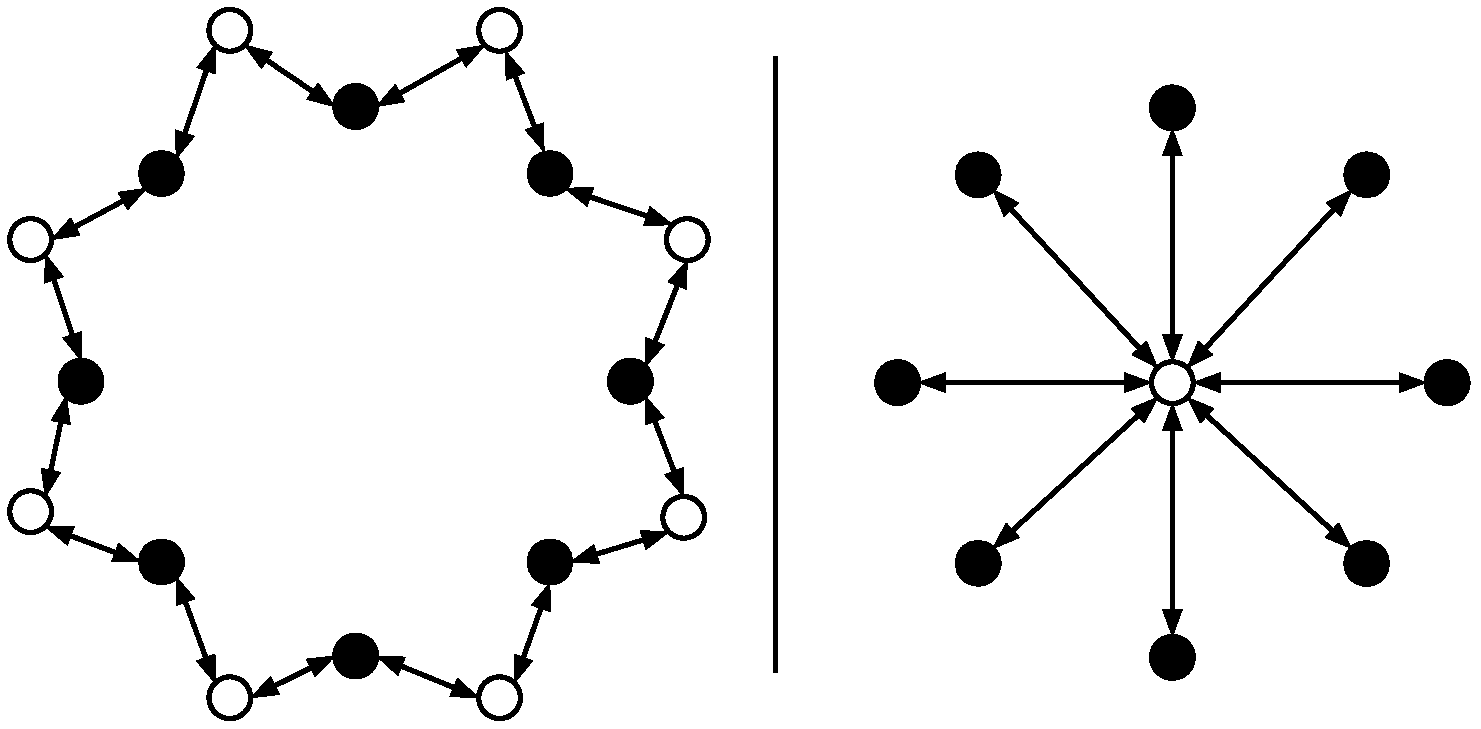
\includegraphics[scale=0.4]{RingVCluster.pdf}
\caption{Two subcomponents formed by process cooperativity. Black dots 
represent processes, and the white dots represent a channel.}
\label{fig:RingVCluster}
\end{figure}

To illustrate this problem, figure~\ref{fig:RingVCluster} visualizes two 
possible components which may occur naturally. On the left we get a ring like
structure, where the dependency of one process is the one to it's right.
We can abstractly envision a data-flow like application which acts like
a token ring network. On the right we have a cluster of processes, all 
communicating with a random other on the same channel. We can envision this
as an abstraction over a single shared resource.

Both the ring and cluster subcomponents would gradually become grouped into a 
KRoC batch. This is optimal for the ring component, no matter how large the 
ring may be. There is nothing to be gained from splitting it into multiple 
batches, and by doing so, we may actually hinder it. However, the cluster 
component may improve if given the chance for more parallelism, this would
depend entirely on the longevity of the processes.
KRoC attempts to account for this by recognizing if there are multiple active
processes in a batch, and splitting an arbitrary one into a new batch (which
ever happens to be at the head of the process queue). 

While this may not be avoidable based on observing structure alone, we may now 
run into an issue. Suppose all processes are active, but run for a length of time under their
designated time quantum. At every preemption, when the size of the batch forces 
a split, we will create a singleton batch which must be reabsorbed after a 
single run. Ignoring the overhead, fairness properties also start to percolate.
Namely, the processes within the batch after being trimmed will get preferential
treatment to the processes in the singleton queue. Especially in the case of 
a single processor. Inevitably, the worst-case scenario for KRoC is below that
of the work-stealing scheduler.

From this we can take that the longevity of a process can effect it's 
cooperativity. In fact, looking at 
definition~\ref{def:degree of cooperativity}, we can apply it to a single 
process too. Now, a \emph{process' degree of cooperativity} can be defined as 
its \emph{frequency} of interaction with a set of channels.
Thus, a cooperativity-conscious scheduler should also want to consider both
the longevity of a process, and which channels it communicates with. This would
give a much more complete picture of cooperativity.

